% Manuscript scaffold: section headers, measured results, and dataset construction.
% Unwritten prose remains in comments rather than appearing as instructions.
\documentclass[letterpaper]{article}
\usepackage[submission]{aaai2027}
\usepackage[hyphens]{url}
\usepackage{graphicx}
\urlstyle{rm}
\def\UrlFont{\rm}
\usepackage{natbib}
\usepackage{caption}
\frenchspacing
\usepackage{booktabs}
\pdfinfo{/TemplateVersion (2027.1)}
\setcounter{secnumdepth}{2}
\title{Target Assignment in Synthetic Tabular Data}
\author{Anonymous Authors}
\affiliations{}
\begin{document}
\maketitle
\begin{abstract}
% Write after the main claims and results are settled.
\end{abstract}

\section{Introduction}
% Motivation, target-assignment question, and bounded contributions.
\section{Related Work}
% Synthetic tabular data, predictive utility, and supervised target assignment.

\section{Target Assignment in Synthetic Tables}
We compare three constructions. A joint generator produces $(\widetilde X,
\widetilde Y)$; the generated-target baseline retains both. Joint relabeling
retains exactly the same $\widetilde X$ and replaces $\widetilde Y$ with
$h(\widetilde X)$, where $h$ is trained on real training data. Features-only
relabeling fits a separate generator to $X$ and assigns targets with the
same labeler. We evaluate CTGAN and TVAE~\citep{xu2019ctgan} and include
the ongoing TabDDPM comparison~\citep{kotelnikov2023tabddpm}.
\subsection{Learning the Target Predictor}
% Labelers, hard classification decisions, and regression predictions.
\subsection{Synthetic-only and Mixed Training}
% Define the two training regimes and the real-only reference.

\section{Experimental Setup}
\subsection{Real-data Benchmark}
The selected benchmark contains Adult, Census KDD, Covertype, MNIST12,
MNIST28, News, and California Housing, with experiment seeds 42 and 43.
Rows are partitioned before fitted preprocessing. Identical feature groups
are kept together, split state 42 is shared across experiment seeds, and
rare-class protection can change the realized partition sizes. Encodings,
scaling, generators, and labelers are fitted on training data. Real
development data select downstream checkpoints; real test data evaluate
the selected checkpoint.

Generators use 500 epochs, batch size 500, and 100,000 synthetic rows.
Mixed training concatenates all real training rows and all synthetic rows.
RF, XGB, and DNN are target predictors. Neural networks
evaluate downstream utility. The TabDDPM comparison uses unconditional
joint and features-only models under this protocol; it is not a replication
of the original paper's conditional classification protocol.

\subsection{Construction of the Simulated Datasets}
The known-distribution benchmark separates prediction from recovery of
the original joint distribution. Each dataset has independent training
and test draws of 10,000 rows, and each synthetic table has 10,000 rows.
Experiment seeds are 42 and 43. CTGAN and TVAE use 300 epochs and batch
size 500. The seven datasets comprise three mixed continuous/categorical
distributions and four categorical Bayesian networks.

\subsubsection{Gaussian, Grid, and Ring}
Each row contains two continuous features $X_0,X_1$, a binary feature $C$,
and a binary target $Y$. Gaussian draws $X_0$ and $X_1$ independently from
$\mathcal N(0,1)$. Grid independently selects each coordinate's center
uniformly from $\{-4,-2,0,2,4\}$, adds Gaussian noise of standard deviation
$0.2$, and divides by $\sqrt{8+0.2^2}$. It has 25 modes on a five-by-five
grid. Ring selects one of eight equally spaced centers on the unit circle,
adds isotropic Gaussian noise of standard deviation $0.2$, and divides
both coordinates by $\sqrt{0.5+0.2^2}$. Its coordinates are dependent.

All three use the same conditional feature and target rules:
\begin{equation}
 C\mid X\sim\mathrm{Bernoulli}\!\left(\sigma(2X_0X_1)\right),
\end{equation}
where $\sigma$ is the logistic function, and
\begin{equation}
 h^*(X,C)=\mathbf 1\{X_1+[1+0.75(2C-1)]X_0>0\}.
\end{equation}
The observed target is $Y=h^*(X,C)\mathbin{\oplus}E$, with independent
$E\sim\mathrm{Bernoulli}(0.10)$ and exclusive-or $\oplus$.
Thus the Bayes accuracy is $0.90$. Conditioning on $C$ changes the
decision boundary, as shown in Figure~\ref{fig:simulated-construction}.

\begin{figure*}[t]
\centering
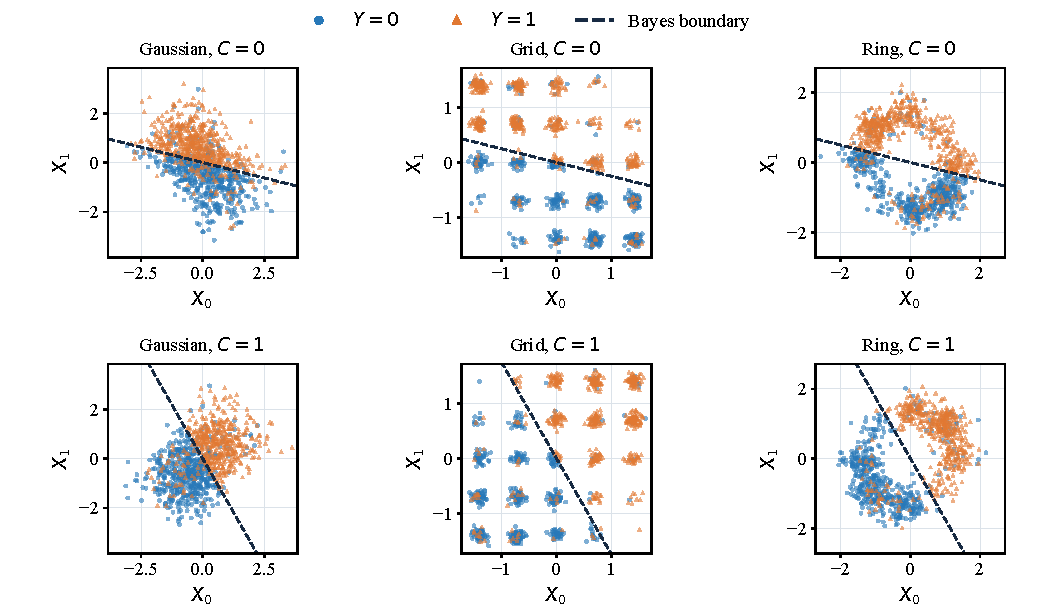
\includegraphics[width=\textwidth]{figures/simulated_construction.pdf}
\caption{Gaussian, Grid, and Ring, conditioned on the binary feature $C$.
Points are original-process rows; circles denote $Y=0$ and triangles
denote $Y=1$. Dashed lines show the Bayes decision boundary. Each dataset
is illustrated with 2,000 saved rows (seed 7), independent of the
benchmark's 10,000-row draws with seeds 42 and 43.}
\label{fig:simulated-construction}
\end{figure*}

\subsubsection{Categorical Bayesian Networks}
Asia, Alarm, Child, and Insurance use the packaged graphs and their
original conditional probability tables. We sample ancestrally from each
network, designate one node as the target (Table~\ref{tab:simulated-schema}),
and observe every other node as a feature. State codes are categorical,
not ordinal. No additional label noise is introduced. Figure~\ref{fig:asia}
shows Asia as an example. Oracle posteriors are computed by enumerating
the target states with the other nodes observed. Bayes accuracy is
estimated by averaging the maximum posterior over independent test features.
\begin{table}[t]
\centering
{\small
\begin{tabular}{lrlr}
\toprule
Network & Features & Target & States \\
\midrule
Asia & 7 & \texttt{dysp} & 2 \\
Alarm & 36 & \texttt{BP} & 3 \\
Child & 19 & \texttt{Disease} & 6 \\
Insurance & 26 & \texttt{Accident} & 4 \\
\bottomrule
\end{tabular}
}
\caption{Categorical Bayesian-network datasets. Every non-target node is observed. Original conditional probability tables define each joint distribution.}
\label{tab:simulated-schema}
\end{table}

\begin{figure}[t]
\centering
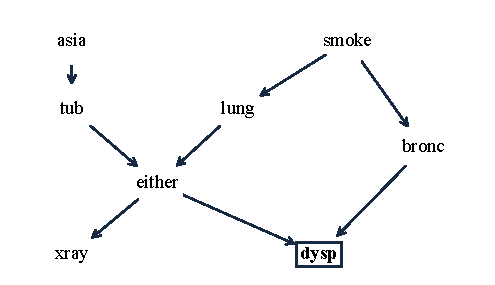
\includegraphics[width=\columnwidth]{figures/asia_graph.pdf}
\caption{The Asia network. The boxed node, \texttt{dysp}, is the target;
all other nodes are observed features. Arrows and conditional probability
tables define the original joint distribution used to sample rows.}
\label{fig:asia}
\end{figure}

\subsection{Evaluation Metrics}
Real-data classification tables report the metric used in the dataset
comparison: binary and macro F1 for Adult and Census KDD, macro F1 for
Covertype, and accuracy for MNIST12 and MNIST28. Regression tables report
$R^2$ and $D^2$ absolute error. $D^2$ is one minus the test MAE divided
by the MAE of the constant test-median predictor. Both metrics are
unscaled; higher is better.

The simulated benchmark reports accuracy against observed targets,
macro F1, and agreement with $h^*$. $L_{\rm syn}$ scores training rows
under the known original joint distribution. $L_{\rm test}$ fits a
normalized density to the training table and scores independent original
test rows; it is a density-refit proxy. Bayesian-network likelihood
reports use $\log(p+10^{-8})$ once on the full joint probability and track
exact-zero support violations separately.

\FloatBarrier
\section{Results on Real Data}
Tables~\ref{tab:real-synthetic} and~\ref{tab:real-mix} compare generated
targets with X-only relabeling in the two training regimes. TabDDPM
results are partial.
\subsection{Generated Targets versus Predicted Targets}
\begin{table*}[!t]
\centering
\setlength{\tabcolsep}{6pt}
\begin{tabular}{@{}lrrrrrrr@{}}
\toprule
\multicolumn{8}{@{}l}{\textbf{(a) Classification (\%)}} \\
\addlinespace
\textbf{Method} & \multicolumn{2}{c}{\textbf{Adult}} & \multicolumn{2}{c}{\textbf{Census KDD}} & \multicolumn{1}{c}{\textbf{Covertype}} & \multicolumn{1}{c}{\textbf{MNIST12}} & \multicolumn{1}{c}{\textbf{MNIST28}} \\
\cmidrule(lr){2-3}\cmidrule(lr){4-5}\cmidrule(lr){6-6}\cmidrule(lr){7-7}\cmidrule(lr){8-8}
 & Binary F1 & Macro F1 & Binary F1 & Macro F1 & Macro F1 & Accuracy & Accuracy \\
\midrule
Real only & 67.45 & \textbf{79.14} & \textbf{55.21} & \underline{75.63} & 50.47 & \textbf{95.63} & \textbf{97.97} \\
\midrule
\multicolumn{8}{@{}l}{\textbf{Baselines: generated targets}} \\
CTGAN & 61.71 & 75.77 & 47.42 & 71.05 & 44.76 & 54.02 & 57.26 \\
TVAE & 56.74 & 72.93 & 47.00 & 71.21 & 43.42 & 92.83 & 94.20 \\
TabDDPM & --- & --- & --- & --- & --- & --- & --- \\
\midrule
\multicolumn{8}{@{}l}{\textbf{Our methods: X-only + predicted targets}} \\
CTGAN-X + RF & 65.63 & 77.87 & 52.75 & 74.66 & 54.16 & 88.83 & 87.95 \\
CTGAN-X + XGB & 66.43 & 78.06 & 54.24 & 75.45 & 50.48 & 90.28 & 88.83 \\
CTGAN-X + DNN & \textbf{68.64} & \underline{78.57} & \underline{54.40} & \textbf{75.74} & \textbf{69.09} & 91.14 & 91.95 \\
\addlinespace
TVAE-X + RF & 65.86 & 77.98 & 48.53 & 72.21 & 46.21 & 92.84 & 94.55 \\
TVAE-X + XGB & 66.91 & 78.47 & 49.92 & 73.13 & 45.59 & \underline{94.20} & 95.89 \\
TVAE-X + DNN & \underline{68.55} & 78.39 & 52.85 & 74.79 & \underline{63.94} & 93.80 & \underline{95.95} \\
\bottomrule
\end{tabular}
\par\medskip
\setlength{\tabcolsep}{16pt}
\begin{tabular}{@{}lrrrr@{}}
\toprule
\multicolumn{5}{@{}l}{\textbf{(b) Regression}} \\
\addlinespace
\textbf{Method} & \multicolumn{2}{c}{\textbf{News}} & \multicolumn{2}{c}{\textbf{Housing}} \\
\cmidrule(lr){2-3}\cmidrule(lr){4-5}
 & $R^2$ & $D^2$ & $R^2$ & $D^2$ \\
\midrule
Real only & -0.0290 & -0.0445 & 0.5125 & 0.2822 \\
\midrule
\multicolumn{5}{@{}l}{\textbf{Baselines: generated targets}} \\
CTGAN & -0.0195 & \textbf{0.0150} & 0.6315 & 0.4136 \\
TVAE & -0.0274 & 0.0049 & 0.7145 & 0.5054 \\
TabDDPM & --- & --- & 0.8020$^{\dagger}$ & 0.6045$^{\dagger}$ \\
\midrule
\multicolumn{5}{@{}l}{\textbf{Our methods: X-only + predicted targets}} \\
CTGAN-X + RF & -0.0003 & -0.0006 & 0.7900 & 0.5857 \\
CTGAN-X + XGB & 0.0000 & -0.0104 & \textbf{0.8195} & \underline{0.6212} \\
CTGAN-X + DNN & 0.0018 & \underline{0.0074} & 0.8039 & 0.6075 \\
\addlinespace
TVAE-X + RF & \underline{0.0026} & -0.0026 & 0.7790 & 0.5732 \\
TVAE-X + XGB & 0.0020 & -0.0319 & \underline{0.8173} & \textbf{0.6217} \\
TVAE-X + DNN & \textbf{0.0102} & -0.0208 & 0.7577 & 0.6061 \\
\bottomrule
\end{tabular}
\caption{Synthetic-only training. Means over seeds 42/43; higher is better for every metric. $D^2$ uses absolute error relative to the test-median baseline. G-X fits generator G to features only, then uses the named labeler. Bold: best; underline: second-best distinct displayed mean, including real-only and ties. $\dagger$: seed 42 only, excluded from ranking; ---: no completed entry in the October 11, 2026, 00:25 Chicago TabDDPM snapshot. TabDDPM X-only results are unavailable. MNIST12 TVAE retains the feature-collision caveat.}
\label{tab:real-synthetic}
\end{table*}

\begin{table*}[!t]
\centering
\setlength{\tabcolsep}{6pt}
\begin{tabular}{@{}lrrrrrrr@{}}
\toprule
\multicolumn{8}{@{}l}{\textbf{(a) Classification (\%)}} \\
\addlinespace
\textbf{Method} & \multicolumn{2}{c}{\textbf{Adult}} & \multicolumn{2}{c}{\textbf{Census KDD}} & \multicolumn{1}{c}{\textbf{Covertype}} & \multicolumn{1}{c}{\textbf{MNIST12}} & \multicolumn{1}{c}{\textbf{MNIST28}} \\
\cmidrule(lr){2-3}\cmidrule(lr){4-5}\cmidrule(lr){6-6}\cmidrule(lr){7-7}\cmidrule(lr){8-8}
 & Binary F1 & Macro F1 & Binary F1 & Macro F1 & Macro F1 & Accuracy & Accuracy \\
\midrule
Real only & 67.45 & \textbf{79.14} & 55.21 & 75.63 & 50.47 & \textbf{95.63} & \textbf{97.97} \\
\midrule
\multicolumn{8}{@{}l}{\textbf{Baselines: generated targets}} \\
CTGAN & 65.17 & 77.69 & 44.69 & 68.42 & 49.61 & 71.88 & 92.77 \\
TVAE & 60.18 & 74.95 & 55.39 & 75.86 & 48.92 & 94.35 & 96.45 \\
TabDDPM & --- & --- & --- & --- & --- & --- & --- \\
\midrule
\multicolumn{8}{@{}l}{\textbf{Our methods: X-only + predicted targets}} \\
CTGAN-X + RF & 66.71 & 78.60 & 55.82 & 76.47 & 57.41 & 92.94 & 95.73 \\
CTGAN-X + XGB & 66.44 & 78.20 & 56.98 & 76.98 & 57.90 & 94.10 & 96.20 \\
CTGAN-X + DNN & \underline{68.62} & 78.36 & 56.99 & 77.10 & \textbf{74.76} & 93.79 & 96.38 \\
\addlinespace
TVAE-X + RF & 65.19 & 77.76 & 56.15 & 76.56 & 54.26 & 93.97 & 95.99 \\
TVAE-X + XGB & 66.84 & 78.56 & \textbf{57.74} & \textbf{77.42} & 55.60 & \underline{94.80} & \underline{96.87} \\
TVAE-X + DNN & \textbf{68.97} & \underline{78.91} & \underline{57.36} & \underline{77.30} & \underline{73.15} & 94.64 & 96.78 \\
\bottomrule
\end{tabular}
\par\medskip
\setlength{\tabcolsep}{16pt}
\begin{tabular}{@{}lrrrr@{}}
\toprule
\multicolumn{5}{@{}l}{\textbf{(b) Regression}} \\
\addlinespace
\textbf{Method} & \multicolumn{2}{c}{\textbf{News}} & \multicolumn{2}{c}{\textbf{Housing}} \\
\cmidrule(lr){2-3}\cmidrule(lr){4-5}
 & $R^2$ & $D^2$ & $R^2$ & $D^2$ \\
\midrule
Real only & -0.0290 & -0.0445 & 0.5125 & 0.2822 \\
\midrule
\multicolumn{5}{@{}l}{\textbf{Baselines: generated targets}} \\
CTGAN & -0.0173 & \underline{0.0241} & 0.6356 & 0.4187 \\
TVAE & -0.0219 & \textbf{0.0360} & 0.6997 & 0.5028 \\
TabDDPM & --- & --- & 0.7998$^{\dagger}$ & 0.5971$^{\dagger}$ \\
\midrule
\multicolumn{5}{@{}l}{\textbf{Our methods: X-only + predicted targets}} \\
CTGAN-X + RF & -0.0020 & 0.0080 & 0.7820 & 0.5877 \\
CTGAN-X + XGB & \textbf{0.0023} & -0.0004 & \textbf{0.8098} & \textbf{0.6157} \\
CTGAN-X + DNN & -0.0005 & 0.0203 & \underline{0.8028} & \underline{0.6083} \\
\addlinespace
TVAE-X + RF & 0.0006 & 0.0019 & 0.7606 & 0.5551 \\
TVAE-X + XGB & -0.0007 & 0.0086 & 0.8002 & 0.6061 \\
TVAE-X + DNN & \underline{0.0014} & 0.0092 & 0.7875 & 0.6007 \\
\bottomrule
\end{tabular}
\caption{Real + synthetic training. Metrics, means, notation, and highlighting follow Table~\ref{tab:real-synthetic}. Mixing concatenates all real training rows and 100,000 synthetic rows. Daggers identify seed-42-only results.}
\label{tab:real-mix}
\end{table*}

\subsection{Contrast Analysis}
We evaluate two contrasts separately in each training regime. Relabeled
minus generated compares predicted targets with generated targets,
averaging equally over CTGAN/TVAE, RF/XGB/DNN, seeds 42/43, and both
relabeled feature sources. Joint minus X-only compares the two feature
sources with predicted targets in both arms, matching generator, labeler,
and seed. TabDDPM is excluded from these contrasts because its matrix
is incomplete.

Classification inference uses one macro-F1 contrast per dataset, with
equal weight for all five tasks (Table~\ref{tab:classification-contrasts}).
The two-sided paired $t$ tests have four degrees of freedom. Confidence
intervals are pointwise 95\%, and $p$ values are unadjusted. The contrast
questions were selected after earlier analyses, so these tests are
exploratory.

Regression tests use matched held-out predictions for each fixed task
(Table~\ref{tab:regression-contrasts}). We average each case's loss over
the specified fits before comparing constructions. Reductions in squared
and absolute error correspond to gains in $R^2$ and $D^2$, respectively.
We use 99,999 paired sign flips, giving identical-feature groups a common
sign, and compare the absolute permuted and observed mean contrasts.
The raw $p$ value is $(b+1)/100{,}000$, where $b$ counts permutations at
least as extreme. These exploratory tests assume independent groups with
sign-exchangeable loss contrasts under the null. They are conditional on
the fitted models and do not estimate variation from retraining.
\begin{table*}[t]
\centering
\setlength{\tabcolsep}{8pt}
\begin{tabular}{@{}llrrr@{}}
\toprule
\textbf{Training} & \textbf{Contrast} & \textbf{Gain (pp)} & \textbf{95\% CI} & \textbf{Raw $p$} \\
\midrule
Synthetic-only & Relabeled $-$ generated & +11.63 & $[+1.33, +21.93]$ & 0.0350 \\
 & Joint $-$ X-only & +0.36 & $[-0.85, +1.56]$ & 0.4575 \\
\midrule
Mix & Relabeled $-$ generated & +6.77 & $[-0.31, +13.85]$ & 0.0566 \\
 & Joint $-$ X-only & +0.14 & $[-0.85, +1.13]$ & 0.7182 \\
\bottomrule
\end{tabular}
\caption{Classification contrasts across Adult, Census KDD, Covertype, MNIST12, and MNIST28. Gains and pointwise 95\% confidence intervals are in macro-F1 percentage points. Each dataset contributes one contrast, after averaging equally over CTGAN/TVAE, RF/XGB/DNN, and seeds 42/43. Raw $p$ values use exploratory two-sided paired $t$ tests across the five dataset contrasts ($df=4$), with no multiplicity adjustment.}
\label{tab:classification-contrasts}
\end{table*}

\begin{table*}[t]
\centering
\setlength{\tabcolsep}{9pt}
\begin{tabular}{@{}llrrrr@{}}
\toprule
\multicolumn{6}{c}{\textbf{(a) $R^2$}} \\
\textbf{Training} & \textbf{Contrast} & \multicolumn{2}{c}{\textbf{News}} & \multicolumn{2}{c}{\textbf{Housing}} \\
\cmidrule(lr){3-4}\cmidrule(lr){5-6}
 & & Gain & Raw $p$ & Gain & Raw $p$ \\
\midrule
Synthetic-only & Relabeled $-$ generated & +0.0246 & $<0.0001$ & +0.1208 & $<0.0001$ \\
 & Joint $-$ X-only & -0.0031 & $<0.0001$ & -0.0015 & 0.0336 \\
\midrule
Mix & Relabeled $-$ generated & +0.0192 & $<0.0001$ & +0.1212 & $<0.0001$ \\
 & Joint $-$ X-only & -0.0010 & 0.0563 & -0.0033 & 1.0000 \\
\midrule
\multicolumn{6}{c}{\textbf{(b) $D^2$ absolute error}} \\
\textbf{Training} & \textbf{Contrast} & \multicolumn{2}{c}{\textbf{News}} & \multicolumn{2}{c}{\textbf{Housing}} \\
\cmidrule(lr){3-4}\cmidrule(lr){5-6}
 & & Gain & Raw $p$ & Gain & Raw $p$ \\
\midrule
Synthetic-only & Relabeled $-$ generated & -0.0178 & $<0.0001$ & +0.1448 & $<0.0001$ \\
 & Joint $-$ X-only & +0.0038 & $<0.0001$ & +0.0036 & $<0.0001$ \\
\midrule
Mix & Relabeled $-$ generated & -0.0208 & $<0.0001$ & +0.1382 & $<0.0001$ \\
 & Joint $-$ X-only & +0.0025 & $<0.0001$ & +0.0066 & $<0.0001$ \\
\bottomrule
\end{tabular}
\caption{Regression contrasts with unadjusted, two-sided paired permutation $p$ values (99,999 group sign flips). Gains are unscaled; positive values favor the first construction. CTGAN/TVAE, RF/XGB/DNN, and seeds 42/43 receive equal weight. Tests use squared error for $R^2$ and absolute error for $D^2$ on 7,929 News and 4,128 Housing test rows. Inference is exploratory and conditional on the fitted models; it does not measure retraining variability.}
\label{tab:regression-contrasts}
\end{table*}


\section{Results under Known Distributions}
\begin{table}[ht]
\centering
{\small
\setlength{\tabcolsep}{2pt}
\begin{tabular}{lrrrrr}
\toprule
Task & Acc. & $\Delta$Acc. & $\Delta h^*$ & $\Delta L_{\rm syn}$ & $\Delta L_{\rm test}$ \\
\midrule
Gaussian & 82.06 & +7.29 & +9.09 & +0.4081 & -0.0195 \\
Grid & 86.27 & +3.61 & +4.39 & +0.2823 & -0.1906 \\
Ring & 87.49 & +2.14 & +2.70 & +0.4261 & -0.0581 \\
Asia & 85.48 & +0.22 & +0.41 & +0.2354 & -0.7728 \\
Alarm & 66.17 & +14.72 & +22.02 & +0.4146 & +0.0009 \\
Child & 82.42 & +5.35 & +7.92 & +0.3816 & +0.0563 \\
Insurance & 90.31 & +4.24 & +4.78 & +0.1158 & +0.0615 \\
\bottomrule
\end{tabular}
}
\caption{Known-distribution benchmark. Acc. is generated-target accuracy (\%), averaged over two generators and two seeds. Changes compare joint relabeling on the same features with generated targets: RF/XGB/DNN, two generators, two seeds (12 changes per task). Accuracy and $h^*$ agreement changes are percentage points. Density changes use native scores; $L_{\rm test}$ is a refit proxy. BN scores use the full-joint epsilon convention.}
\label{tab:oracle}
\end{table}

% Interpret utility, Bayes agreement, and the two density scores separately.
\subsection{Predictive Utility and Bayes Agreement}
% Full method comparisons and paired joint-target replacement effects.
\subsection{Joint-distribution Fidelity}
% Conditional noise, support violations, and density-refit behavior.

\section{Discussion}
\subsection{When Does Target Replacement Help?}
% Explain task-level heterogeneity without selecting labelers on test scores.
\subsection{Does the Generator Need to Model the Target?}
% Compare joint and features-only sources after fixing the labeler.

\section{Limitations}
The two experiment seeds share real-data partitions, and MNIST12 and
MNIST28 are related tasks. The corrected MNIST12 TVAE data retain the
documented exact feature-collision caveat; train-only fitting does not
establish that every test feature vector is unseen. Hard relabeling does
not reproduce independent target noise. Density-refit scores depend on
the specified estimators. The TabDDPM matrix is incomplete.

\section{Conclusion}
% Write once the claims and the complete generator comparison are settled.
\bibliography{references}
\end{document}
